\section{Results}
\label{sec:results}

\subsection{Taxonomy coverage and episode structure}

% claim: C01
All ten constructs received direct support in the selected register. Documentation and support appeared in 48 of 55 selected threads, and knowledge packaging appeared in 32. These values reflect deliberate cross-cutting coding and purposive selection. They establish that B1 and B10 modify many technical discussions; they do not estimate the proportion of laboratory-automation failures caused by either condition. B2 through B9 produced more discriminating technical patterns. The episode subset separated interface access from platform state, physical representation from validation, observability from recovery, and AI generation from downstream evidence.

Direct-support and primary-code counts are reported in Supplementary Table~S1. The taxonomy's main structural result concerns boundaries. Driver discussions often concern the transition from a nominally available component to an executable interface. Version-control discussions concern the transition from source files to an identified deployment. Labware threads concern the transition from a software resource object to a physically portable definition. Logging discussions concern the transition from observations to reconstructable evidence. Recovery incidents concern the transition from an interrupted software plan to a verified physical state. Testing and AI discussions concern the transition from a generated or simulated object to a claim about experimental performance.

\subsection{Field-level metrics}

\begin{table}[t]
\centering
\caption{Bounded pilot metrics. Each row has a distinct unit and denominator.}
\label{tab:headline-metrics}
\begin{threeparttable}
\begin{tabularx}{\linewidth}{@{}L r l L@{}}
\toprule
Construct & Result & 95\% Wilson & Unit and denominator \\
\midrule
B2 Integration accessibility & 63.9\% & -- & 6 device--interface cases \\
B3 Deployment manifest & 54.2\% & -- & 3 deployment objects; 24 applicable cells \\
B4 Physical definitions & 67.0\% & -- & 4 resource definitions \\
B5 Observability & 52.5\% & -- & 4 execution/diagnostic cases \\
B6 Preflight preventability & 66.7\% & 20.8--93.9\% & 3 definite scenarios of 4 eligible \\
B7 Constraint discovery & 87.5\% & 52.9--97.8\% & 8 incomplete fields of 13 \\
B8 Fully aligned claims & 33.3\% & 9.7--70.0\% & 6 bounded claims \\
B9 Core context expansion & 2.0$\times$ & -- & 5 opening classes \\
B10 Actionable public outcome & 41.7\% & 19.3--68.0\% & 12 documentation cases \\
\bottomrule
\end{tabularx}
\begin{tablenotes}[flushleft]\footnotesize
\item Results demonstrate operationalization in selected cases. They do not estimate forum-wide or industry-wide rates.
\item Wilson intervals are descriptive uncertainty for the stated denominator, not population inference. A dash marks a row whose result is a mean of ordinal component scores or a ratio rather than a proportion, for which a binomial interval would be undefined.
\item Component means are taken over known cells only; unknown cells are excluded rather than scored as zero.
\end{tablenotes}
\end{threeparttable}
\end{table}


\begin{figure}[tp]
  \centering
  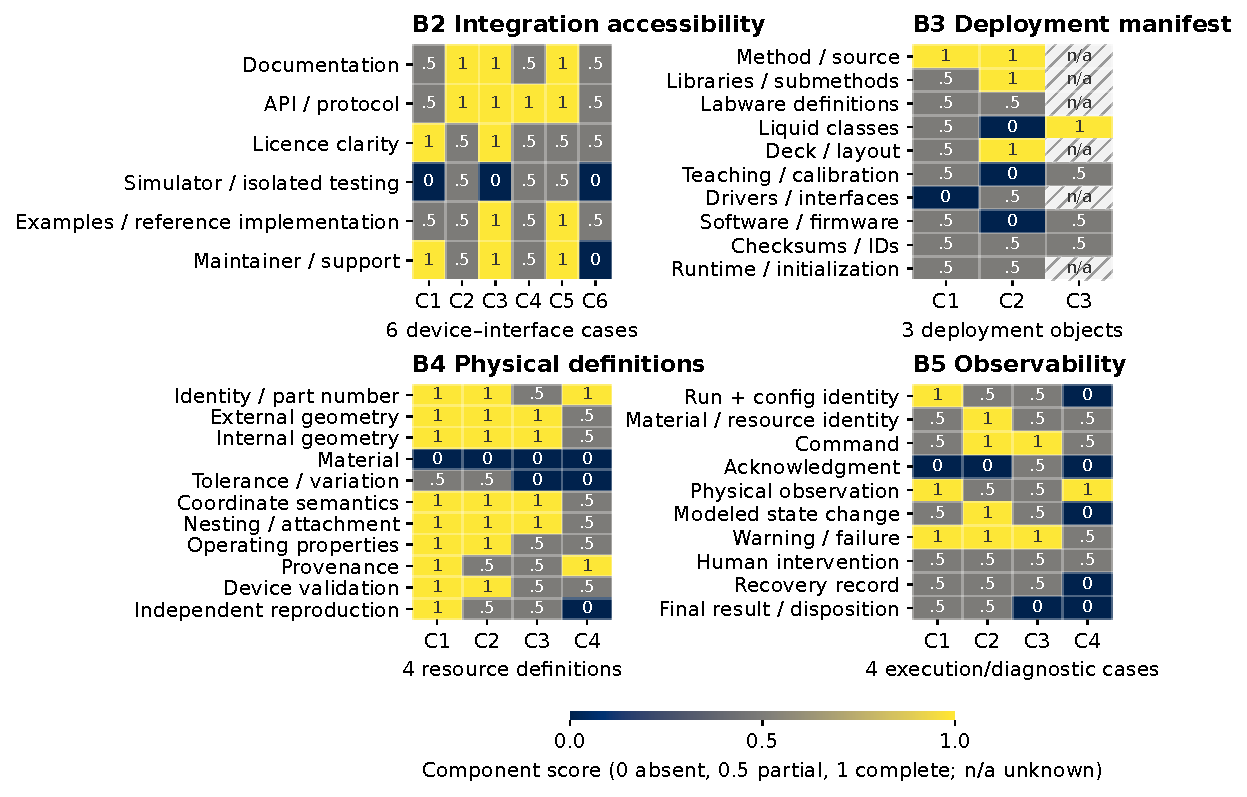
\includegraphics[width=\linewidth]{figures/component_heatmap.pdf}
  \caption{Component-level scores behind the four completeness metrics, with one row per scored field and one column per coded case. Each cell is absent (0), partial (0.5), or complete (1); hatched cells marked \emph{n/a} are outside the case's scope and are excluded from that case's denominator. The four panels have separate case sets and separate field sets, so the panel means are not comparable to one another and do not form a common system-performance scale.}
  \label{fig:component-heatmap}
\end{figure}

The mean Integration Accessibility Score was 63.9\% across six device--interface cases. Documentation averaged 75.0\%, API or protocol access averaged 83.3\%, and simulator or isolated testing averaged 25.0\%. Two cases scored at least 75\%, and three produced a positive public implementation, current interface answer, or structured development pathway. The strongest open case combined a host-independent public API, executable example, and identifiable maintainer. The weakest cases involved inaccessible licensing, missing test surfaces, obsolete tools, model-specific register maps, or support paths that could not resolve the full integration.

Mean Reproducibility Manifest Completeness was 54.2\% across three deployment objects. Only 20.8\% of applicable case--field cells were fully bound. A further 62.5\% were partially represented, which means the field was discussed without an immutable identity covering the execution context. Method source was the strongest field. Teaching or calibration, driver identity, software and firmware versions, and runtime initialization remained weak. The Fluent version-control incident provides the clearest boundary failure. A broad directory included an actively maintained recovery workspace, so a source-control restoration was overwritten by runtime behavior \cite{forum_tecan_git}. The incident demonstrates why source state and active recovery state require separate management.

% claim: C08
Mean Physical Definition Completeness was 67.0\% across four resource cases, with a median evidence grade of 2.5 on the five-level scale from unspecified through independently reproduced. Two cases included explicit device validation, and one reached independent cross-user reproduction. The tip post-mortem received the highest grade because another user reproduced the failure, four causes were isolated, corrections were merged, and the process was documented publicly \cite{forum_tip_postmortem}. Material properties and tolerance or manufacturing variation were the weakest recurring fields. The result suggests that geometry receives more community attention than physical variability.

Mean Observability Coverage was 52.5\% across four execution and diagnostic cases. Two cases localized the first consequential divergence. None fully recorded final material or result disposition. Warning and failure evidence was the strongest field. Explicit acknowledgement, recovery, and final disposition were weakest. The automation-report discussion proposed rich run fields spanning method versions, reagent lots, worklists, third-party states, liquid heights, temperature, humidity, and recoveries \cite{forum_automation_report}. The TADM discussion showed the complementary limitation. Pressure curves were available, while starting volume, tip reuse, full aspiration settings, and independent transfer measurement remained incomplete \cite{forum_tadm}. Rich telemetry without linked context did not support a definitive transfer claim.

\subsection{Partial execution and recovery}

% claim: C02
Four partial-execution scenarios were coded for preflight detectability. Two model-level failures were clearly detectable before the first irreversible action. A hardware crash was not plan-preflight preventable. A bounded software-error scenario included successful return-to-source handling through a custom abort routine, although the public record did not establish whether its triggering error was knowable before aspiration \cite{forum_return_volume}. The complete-case Preflight Preventability Rate was therefore $2/3=66.7\%$. Treating the indeterminate case as non-preventable or preventable produced a sensitivity interval from 50.0\% to 75.0\%. The Wilson interval for two successes in three definite scenarios was 20.8\%--93.9\%, which communicates the small denominator more faithfully than the point estimate alone. Supplementary Figure~S3 shows the four scenarios beside the rate, its interval, and its sensitivity bounds.

The composite-transfer incident exposes the mechanism. Tip pickup and aspiration completed before a destination-lid state error prevented dispensing \cite{forum_error_catching}. The failure had a software location and a physical consequence. Valuable liquid remained in tips, source-volume state had changed, and ordinary method restart could duplicate or invalidate actions. Full-sequence validation could detect the modeled state conflict before dispatch. Recovery still required a record of completed actions, material in transit, operator intervention, and final disposition.

\subsection{Scheduling constraint discovery}

% claim: C03
The scheduling toy problem included devices, capacities, task quantities, durations, transfer time, and release times. It partially specified precedence, storage, timing preferences, and priorities. It omitted sample stability, interruptibility, terminal disposition, and failure policy. Weighted opening completeness was 53.8\%, strict completeness was 38.5\%, and field coverage was 69.2\%. Seven of eight incomplete requirement classes were surfaced in replies, producing an 87.5\% discovery rate. None received a definitive scenario-specific value, producing a 0\% resolution rate and an 87.5 percentage-point discovery--resolution gap \cite{forum_scheduling_toy}.

\begin{figure}[tp]
  \centering
  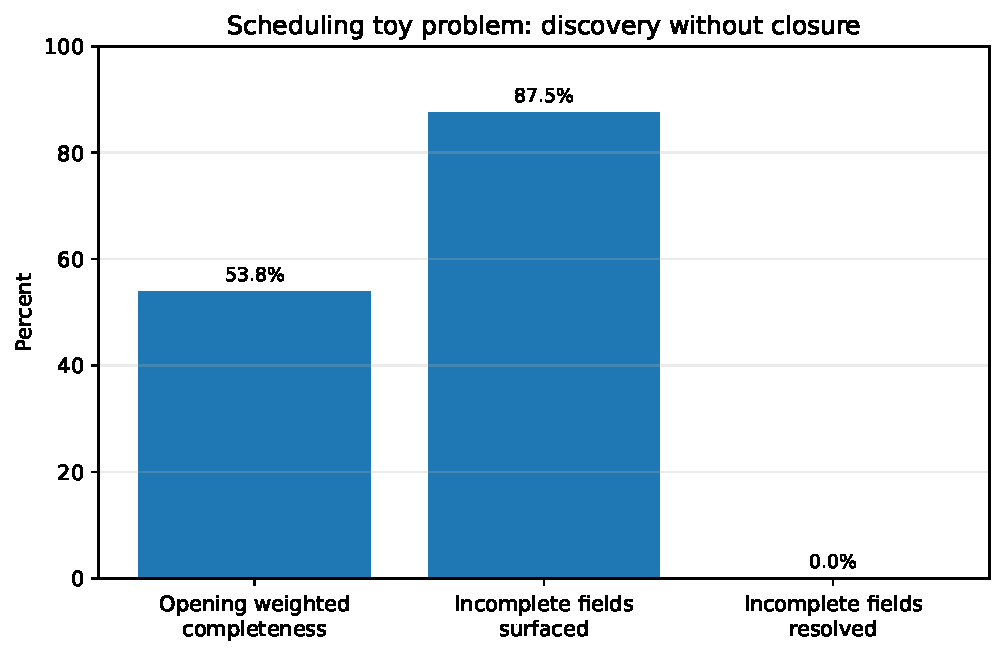
\includegraphics[width=0.86\linewidth]{figures/discovery_resolution.pdf}
  \caption{Each scheduling requirement class at three stages of the single analyzed discussion: specification in the opening post, surfacing in replies, and resolution to a scenario-specific value. The discussion surfaced seven of the eight incomplete classes and resolved none of them, so the constraint set was clarified without producing a fully specified benchmark instance.}
  \label{fig:discovery-resolution}
\end{figure}

This result captures a positive community function. The discussion identified which scientific and operational facts determine feasibility. It also shows why scheduler comparisons need a common evaluation object. Makespan, utilization, waiting time, or replanning quality become interpretable only after the scenario specifies sample windows, permitted storage, interruptibility, disposal, priorities, and failure behavior.

\subsection{Test--claim alignment and AI validation}

% claim: C09
Mean element completeness across six bounded test claims was 73.3\%. Two claims fully aligned object, environment, acceptance rule, observed evidence, and scope. Five were at least partially aligned. The strongest aligned cases were the cross-machine tip-definition post-mortem and the VerisFlow result after its wording was restricted to simulation-trace agreement. A proposed contamination experiment was incomplete because no executed evidence or reconciled acceptance threshold was reported. TADM pressure evidence was partial because the observed curves lacked complete starting conditions and an independent transfer measure. Supplementary Figure~S2 resolves each claim into its five elements.

% claim: C05
The VerisFlow post reported 92 matching traces from 100 randomly generated worklists. The corresponding Wilson interval was 85.0\%--95.9\% \cite{forum_verisflow}. The deepest quantitatively supported stage was simulation-trace agreement. No dry hardware, wet transfer, or assay rate was reported in the analyzed discussion. Supplementary Figure~S1 binds the reported denominator to that validation stage and marks later physical stages as unreported.

% claim: C04
The AI method-writing thread contained five opening context classes: operation vocabulary, volume, position, speed, and hardware boundaries \cite{forum_ai_method}. Replies added ten core execution classes and seventeen broader deployment classes. The core Context Expansion Ratio was 2.0, the broad ratio was 3.4, and a conservative ontology that merged related concepts produced 2.2. The added classes included physical and biological behavior, sample consequence, human observation, missing method context, combinatorial interactions, third-party devices, LIMS-specific data handling, collaboration, regulatory context, and wet-process optimization. These ratios quantify requirements elicitation and do not represent model failure probabilities.

\subsection{Documentation and public outcomes}

% claim: C10
Twelve documentation-centered cases were coded by subtype. Five received a fully actionable public resolution, ten received at least a partial resolution, and three partly migrated toward private contact. Detail or completeness was the strongest subtype, followed by examples, support responsiveness, discoverability, and terminology. Complete absence was least frequent. The common problem was therefore not an empty documentation landscape. It was a fragmented path in which reference material existed inside software, behind commercial access, in an obsolete version, without a working example, or without clear maintenance ownership.

Positive cases were substantial. A Hamilton HSL discussion surfaced installed reference material and clarified the boundary between public documentation, training, and source review \cite{forum_hsl_learning}. A PyLabRobot thread documented local builds and a page-level edit path \cite{forum_plr_docs}. Public vendor responses clarified current APIs and file semantics. These outcomes show that the forum can convert opaque knowledge into reusable guidance. Partial and private migration still limit public canonicalization.

\subsection{Pairwise technical relationships}

\begin{table}[t]
\centering
\caption{Strongest pairwise technical-code associations in the purposive evidence register.}
\label{tab:associations}
\begin{threeparttable}
\begin{tabular}{@{}lrrr@{}}
\toprule
Pair & Overlap & $\phi$ & Lift \\
\midrule
B5--B6 & 8/55 & 0.452 & 2.353 \\
B5--B8 & 11/55 & 0.424 & 1.873 \\
B2--B7 & 8/55 & 0.409 & 2.157 \\
B4--B8 & 8/55 & 0.316 & 1.781 \\
B8--B9 & 4/55 & 0.302 & 2.316 \\
\bottomrule
\end{tabular}
\begin{tablenotes}[flushleft]\footnotesize
\item Associations are descriptive. Multi-label coding, purposive selection, and thread dependence preclude population or causal interpretation.
\end{tablenotes}
\end{threeparttable}
\end{table}


\begin{figure}[tp]
  \centering
  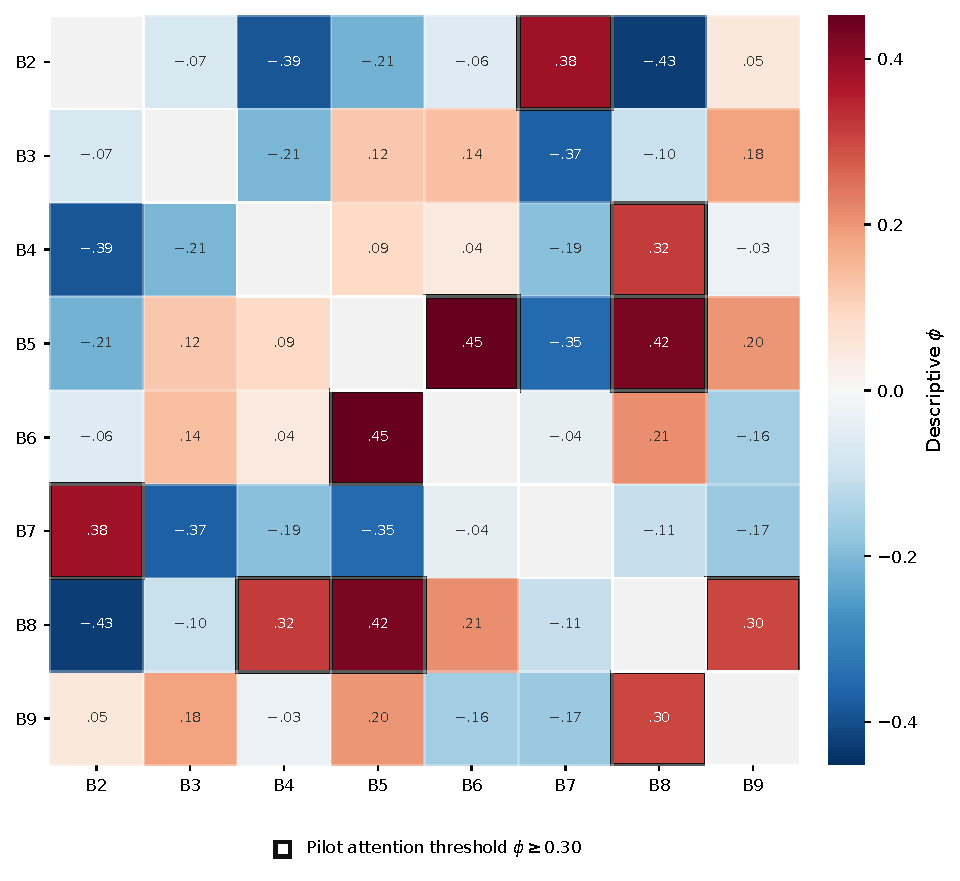
\includegraphics[width=0.82\linewidth]{figures/associations.pdf}
  \caption{All 28 pairwise phi coefficients among the technical constructs B2--B9, computed on the 55 selected threads. Outlined cells exceed the pilot attention threshold $\phi \geq 0.30$. The coefficients describe co-occurrence within a purposively selected register; they are not tests of association in a population, and negative values are not interpreted as technical antagonism because forum structure and primary-topic coding can separate codes on their own.}
  \label{fig:associations}
\end{figure}

% claim: C06, C07
Observability and recovery formed the strongest pair, with overlap in 8 of 55 threads, $\phi=0.452$, and lift $=2.353$. Observability and validation followed with $\phi=0.424$. Interface accessibility and scheduling had $\phi=0.382$. Physical definitions and validation had $\phi=0.316$. Validation and AI context had $\phi=0.302$, although this result was sensitive because B9 contained only five threads. All five coefficients remained positive under one-thread overlap sensitivity. Negative and zero associations were not interpreted substantively because forum categories, selection, and primary-topic structure can create separation without technical antagonism.
